\section{Aufbau}
Zentrale Elemente für den Versuch sind die zwei Laser welche auf eine Platte montiert sind. Die Platte selbst ist durchsichtig,
es bietet sich also an, einer vielzahl an Messsskalen variabel unter den Aufbau zu legen um so mehrere Messereihen mit der gleichen 
Konfiguartion zu messen. \\
Die Laser selbst sind aufeinander monitiert, mit folglich horizontal versetzten aber parallelen Strahlen. Für verschiedene
Winkel bleibt es nun frei den Laser selbst oder das Medium mitsamt Messsskaler zu verschieben. Im uns dagegebenen Versuch 
ist eben der Laseraufbau variabel auf einem Kreisbogen mit einer Ausrichtung die immerzu auf das Medium zeigt. Der Laserstrahl 
bewegt sich also in Richtung des Normalenvektors des Kreisbogen bei entsprechender Position. \\
Im laufe der Durchführung wird sowohl Reflexion als auch Beugung beobachtet, es gilt also Werte jeweil hinter oder vor dem Medium 
aufzunehmen. Im Falle von Reflexion ist ein sogenannter Reflektionsschirm auf die Platte fixiert. Dieser bietet Halt für eventuelle
Transmissionsschirme oder allgemeinen Schutz vor dem Laserlicht.

\begin{figure}
    \centering
    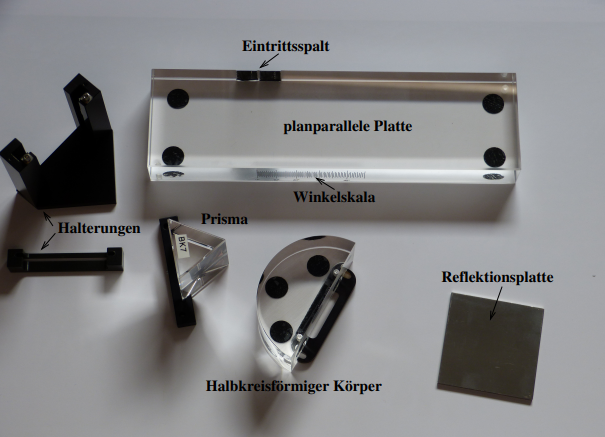
\includegraphics[width=0.5\textwidth]{bilder/teile.png}
    \caption{Bildaufnahme der verschieden Elemente die im Verlaufe des Versuchs V400 zu benutzten sind. \cite{skript}} 
    \label{fig:figskizze1}
\end{figure}

Das optische Material, welches im Mittelpunbkt des Kreisbogen zu platieren ist, bedient sich verschiedener Elemente um 
die jeweils gesuchten Messwerte zu bestimmen. Bei manchen dieser Medien empfiehlt es sich eine enstprechende Haltung zu benutzen.
\begin{description}
    \item Planparallele Platte: \\
    Dieses Element misst eine Dicke von $d = \SI{5.85}{\cm}$, weist auf einer Seite einen Eintrittssplat und auf der anderen 
    eine Winkelskala auf.
    \item Prisma \\
    Das Prisma besteht aus Kronglas und ist charakterisiert durch einen brechenden Winkel $\gamma = 60 \si{\degree}$.
    \item Reflektionsplatte \\
    Um das Reflexionsgesetz zu verifizieren muss das Laserlicht nahezu perfekt refelektiert und anschließend der Winkel
    gemessen werden. Dazu wird die sogenannte Reflektionsplatte benutzt die das Licht mit einem Reflektionskoeffizienten $R= 1$
    reflektiert.
\end{description}



\section{Durchführung}








